\documentclass[landscape, 12pt]{report}

\usepackage{ptext}
\usepackage{lipsum}
\input{Boostan-UserManual}
\usepackage{graphicx}
\usepackage{tabularx}


\newword{Abstraction}{Abstraction}
{انتزاع}{}

\newword{Abstract}{Abstract}
{انتزاعی}{}

\newword{AbsoluteMinimum}{Absolute Minimum}
{کمینه مطلق}{}


\newword{AcceptableCell}{Acceptable Cell}
{سلول پذیرفتنی}{سلول‌های پذیرفتنی}

\newword{AccessBurst}{Access Burst}
{توده دسترسی}{توده‌های دسترسی}


%%% S
\newword{Sample}{Sample}
{نمونه}{نمونه‌ها}

\newword{SamplePath}{Sample Path}
{نمونه مسیر}{}

\newword{SampleSpace}{Sample Space}
{فضای نمونه}{فضای نمونه‌ها}
\newacronym{ACK}{ACK}{Acknowledgement}

\newacronym{ACI}{ACI}{Application Control Interface}

\newacronym{ACIR}{ACIR}{Adjacent Channel Interference Ratio}

\newacronym{ACLC}{ACLC}{Adaptive Configuration of Logical Channels}

\newacronym{ACLP}{ACLP}{Adjacent Channel Leakage Power}

\title{مفهوم
	ORAN
	در شبکه های نسل پنج
}
\type{
 درس آشنایی با شبکه های تلفن همراه }
\author{غزل عربعلی - 97521396، بهاره کاوسی نژاد - 99431217}
\logofile{Pic/IUST}


\begin{document}



\pagenumbering{gobble}
\maketitle
\pagenumbering{arabic}
\chapter*{مقدمه}

\section*{تحولی در معماری
	  \lr{RAN}
	  }
به شکل یک (\ref{fig:site}) که در سمت چپ صفحه مشاهده می‌شود سایت گویند. سایت ها برای ارائه پوشش بی سیم
 (
 \lr{Wireless Coverage}
 ) به کاربران در یک منطقه جغرافیایی خاص قرار می‌گیرند.
\begin{figure}[ht]
	\centering
	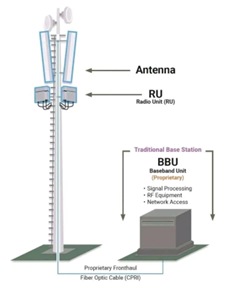
\includegraphics[height=.3\linewidth]{Pic/Picture1}
	\caption{سایت}
	\label{fig:site}
\end{figure}
قرار گیری مولفه های
 \lr{RAN}
   مانند سایت که شامل سلول های زیادی است برای اطمینان از دسترسی قابل اعتماد و ثابت             (
   \lr{Reliable \& Consistent}
   ) کاربران به خدمات شبکه بسیار مهم است. به همین جهت هنگام برنامه ریزی برای استقرار شبکه دسترسی رادیویی، اپراتورهای شبکه عوامل مختلفی را در نظر می گیرند مانند
   \begin{itemize}
   	\item تراکم جمعیت،
   	\item توپوگرافی که به معنای ویژگی ها و خصوصیات سطح زمین در یک منطقه خاص است،
   	\item تراکم ساختمان ها و
   	\item الگوهای ترافیکی در یک منطقه تحت پوشش
   \end{itemize}
چرا که به طور مثال برای دسترسی بهتر کاربران با توجه به آرایش ترافیکی گاهاً به صورت داینامیک
 \lr{Config}
  شبکه را در طول روز تغییر می‌دهند. با تحلیل پارامترهای نام برده شده و دیگر پارامترها اپراتور های شبکه می توانند مکان بهینه و پیکربندی
   \lr{RAN}
    را  با هدف پوشش و ظرفیت حداکثری تعیین کنند. به طور کلی مکان قرارگیری
     \lr{RAN}
      کارایی کلی شبکه را نیز تحت تاثیر قرار می‌دهد.در نتیجه برای داشتن پوشش دهی و
       \lr{Mobility}
        باید از استراتژی برای قرار دادن
         \lr{RAN}
          استفاده کنیم.


\chapter*{اجزای شبکه مخابرات بی سیم}
اجزای شبکه مخابرات بی سیم از ۳ جزء اصلی تشکیل شده است (شکل \ref{fig:Wireless_Telecommunications_Systems}) که یکی
 \lr{User Terminal}
   یا
  \lr{User Equipment}
   و یا
    \lr{Mobile Station}
     که در نسل ۲ از این اصطلاح استفاده می شد، دیگری
      \lr{RAN}
        و آخرین جزء
         \lr{Core Network}
          خواهد بود.
          
          
\begin{figure}[ht]
	\centering
	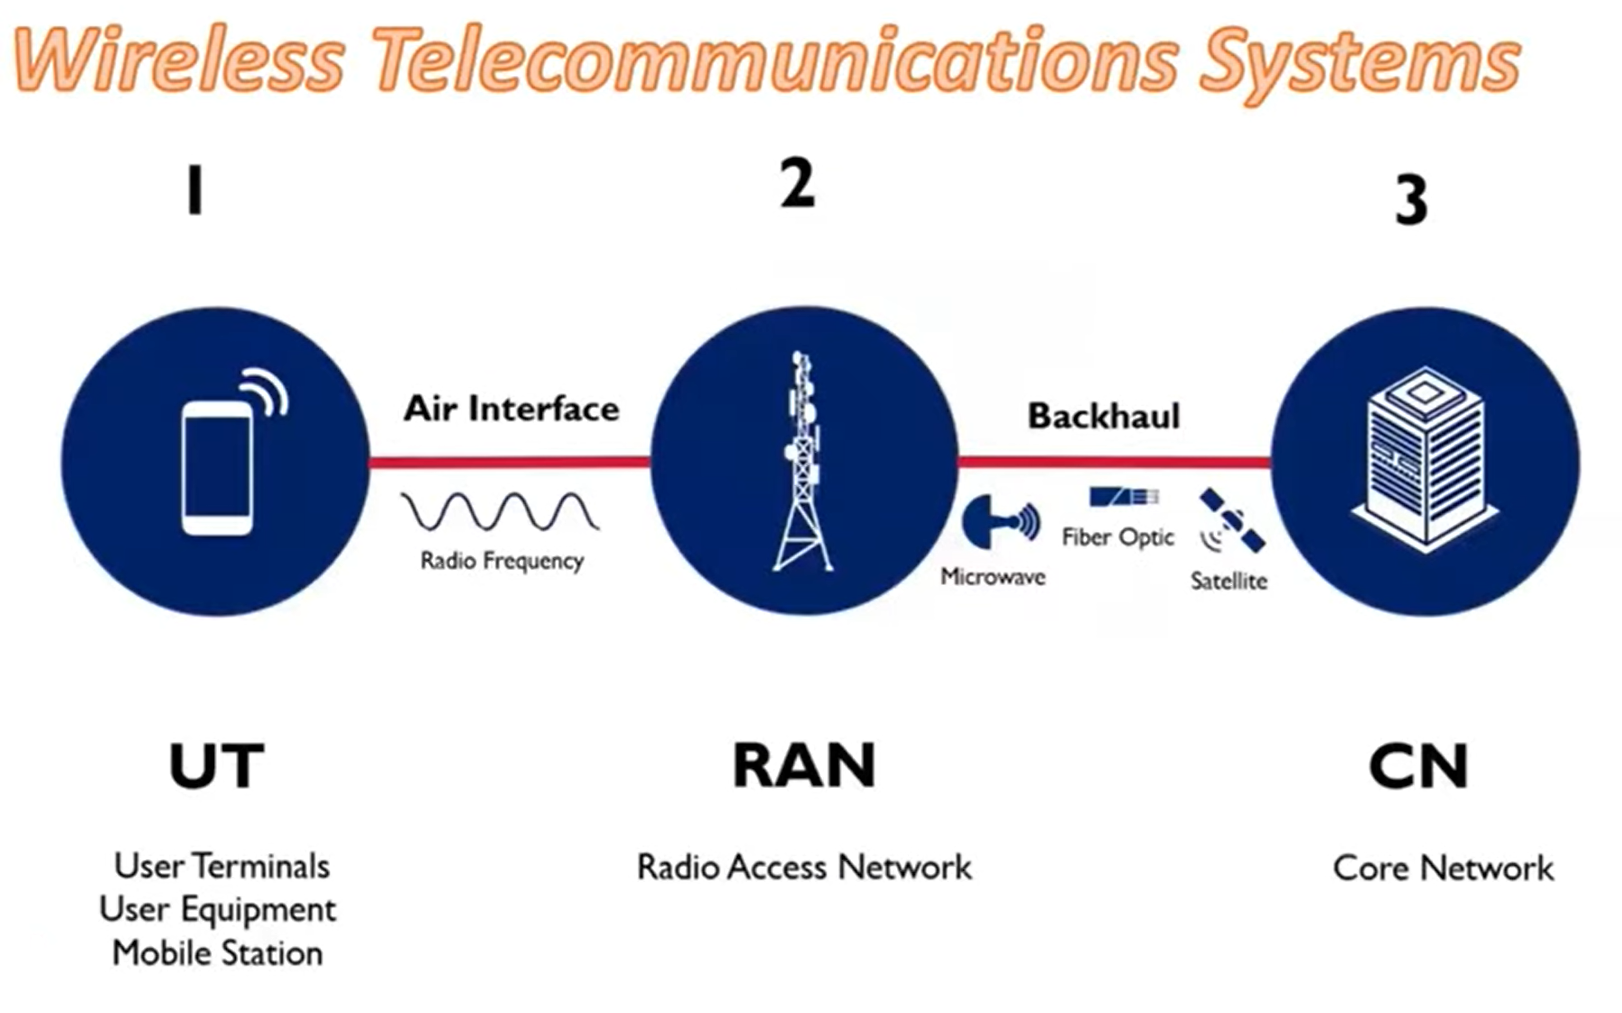
\includegraphics[width=.6\linewidth]{Pic/Wireless_Telecommunications_Systems}
	\caption{اجزای شبکه مخابرات بی سیم}
	\label{fig:Wireless_Telecommunications_Systems}
\end{figure}
وظیفه ناحیه
 \lr{RAN}
  فراهم کردن ارتباط یا
   \lr{Connection Stable}
    برای دستگاه های تلفن همراه است. اگر بخواهیم از ۳ جزء اصلی در
     \lr{Traditional RAN}
      ها نام ببریم میتوان از آنتن،
       \lr{RRU}
        و
         \lr{BBU}
          نام برد. ارتباط میان
            \lr{user terminal}
             و ناحیه
              \lr{RAN}
               از طریق
               \lr{air interface}
                و به صورت
                  \lr{wireless}
                   و با استفاده از پروتکل
                    \lr{AS(Access Stratum)}
                     است که در دیالوگ ها و ارتباط میان دیوایس‌ها و زیر ساخت رادیویی شبکه من جمله
                      \lr{eNodeB}
                       در نسل ۴ و
                        \lr{gNodeB}
                         در نسل ۵ به کار می‌رود . از مجموعه فرکانس های مختلفی جهت برقراری این ارتباط میان ناحیه
                          \lr{RAN}
                           و
                            \lr{User Terminal}
                             استفاده می‌شود که آن را فرکانس رادیویی می‌خوانیم. ناحیه
                              \lr{RAN}
                               از طریق لینک
                                \lr{backhaul}
                                که ترافیک داده از
                                 \lr{RAN}
                                  را به هسته شبکه منتقل می‌کنند به 
                                  \lr{Core Network}
                                   متصل شده اند. 
هسته شبکه وظایف مختلف و مهمی را بر عهده دارد من جمله
 \lr{Routing}
  بین شبکه‌های مختلف،
   \lr{Call}
   ،
    \lr{Message}
    ،
     \lr{USSD}
     ،
      \lr{Internet}
       و به صورت کلی
        \lr{data service}
         ها و ۳ راه اتصال
          \lr{RAN}
           به
            \lr{Core Network}
             وجود دارد که می‌تواند
              \lr{fiber optic}
               یا
                \lr{microwave}
                 باشد و اگر مشکلاتی از در فاصله زیاد و انحنای زمین و ... وجود دارد میتوان از 
                 \lr{Satellite}
                   استفاده کرد.


\section*{بررسی 
\lr{RAN}
به صورت دقیق تر
}
حال به بحث دقیق تر درباره
 \lr{RAN}
  می
  پردازیم:
مکان قرارگیری این ناحیه به صورت خیلی گسترده ای توزیع شده است. چرا در که تمامی نواحی وظیفه برقراری ارتباط و پوشش دهی بدون وقفه و اختلال را دارد.
این ناحیه به طور مداوم از نسل اول تا نسل پنجم تکامل یافته است اما برخی از اجزای ضروری آن باقی مانده اند مانند آنتن که سیگنال الکتریکی را به امواج رادیویی تبدیل می‌کند و بالعکس.
 \lr{RU}
  یا
   \lr{Radio Unit}
    که وظیفه آن استفاده از باند های فرکانسی و سطوح توان مناسب است.
     \lr{BBU}
      یا
       \lr{BaseBand Unit} 
       که سیگنال هارا پردازش می‌کند و این بخش شامل واحد های نرم‌افزاری و سخت‌افزاری جهت برقراری ارتباط بی‌سیم از طریق امواج رادیویی است.
برای ناحیه
 \lr{RAN}
  در نسل های مختلف نامگذاری ها متفاوتی وجود دارد که در تصویر \ref{fig:RAN_Generations} مشاهده می‌کنیم. همان طور که دیده می شود، در نسل پنج، به آن 
  \lr{NG-RAN}
  (
  \lr{New}
  	یا
  	\lr{Next Generation RAN}
  )
  می گویند.
  \begin{figure}[ht]
  	\centering
  	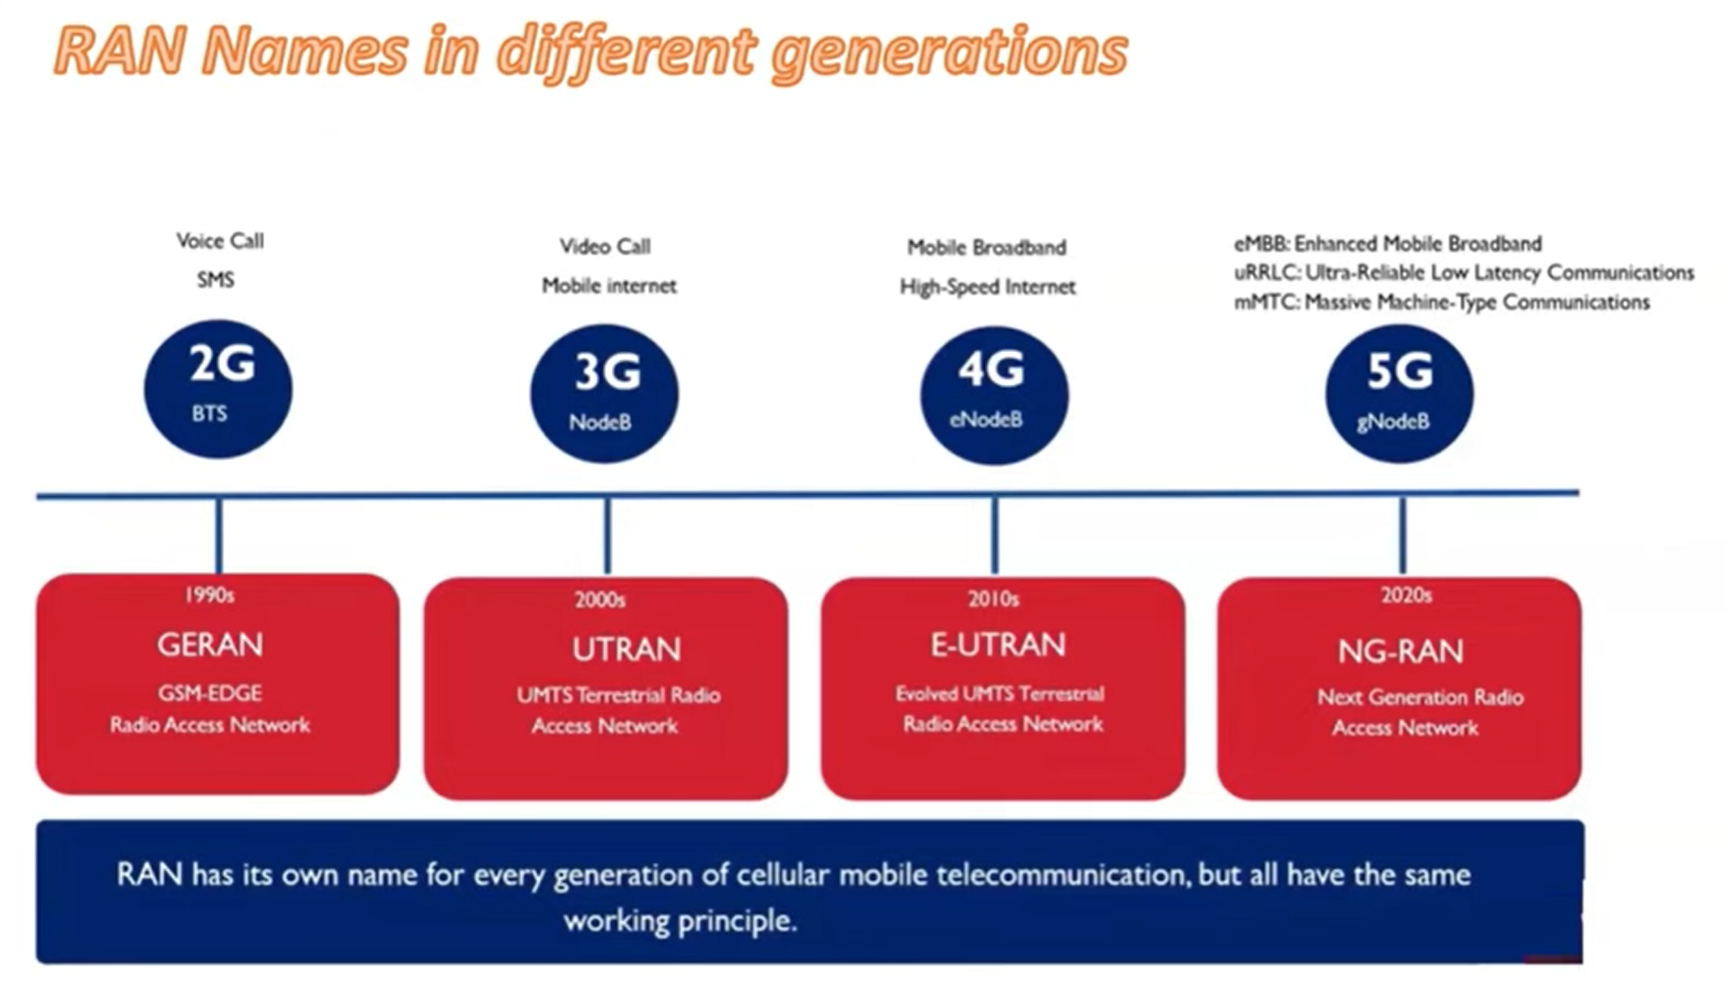
\includegraphics[width=.6\linewidth]{Pic/RAN_Generations}
  	\caption{نسل های مختلف
  		\lr{RAN}
  	}
  	\label{fig:RAN_Generations}
  \end{figure}
  
  همانطور که در شکل \ref{fig:Baseband_Unit} دیده می شود، در 
  \lr{Traditional RAN}
  ،
   \lr{Baseband}
     در زیر برج مانندی قرار دارد و روی برج
      \lr{RRU}
       و آنتن نصب شده‌اند. و این واحد مسئولیت سیگنال های
        \lr{Baseband}
         را بر عهده دارد و در یک کابینی به نام
          \lr{Equipment Room}
           قرار دارد و به وسیله فیبر نوری به
            \lr{RRU}
             که روی برج مانند نصب شده است متصل می‌شود. 
 \begin{figure}[ht]
 	\centering
 	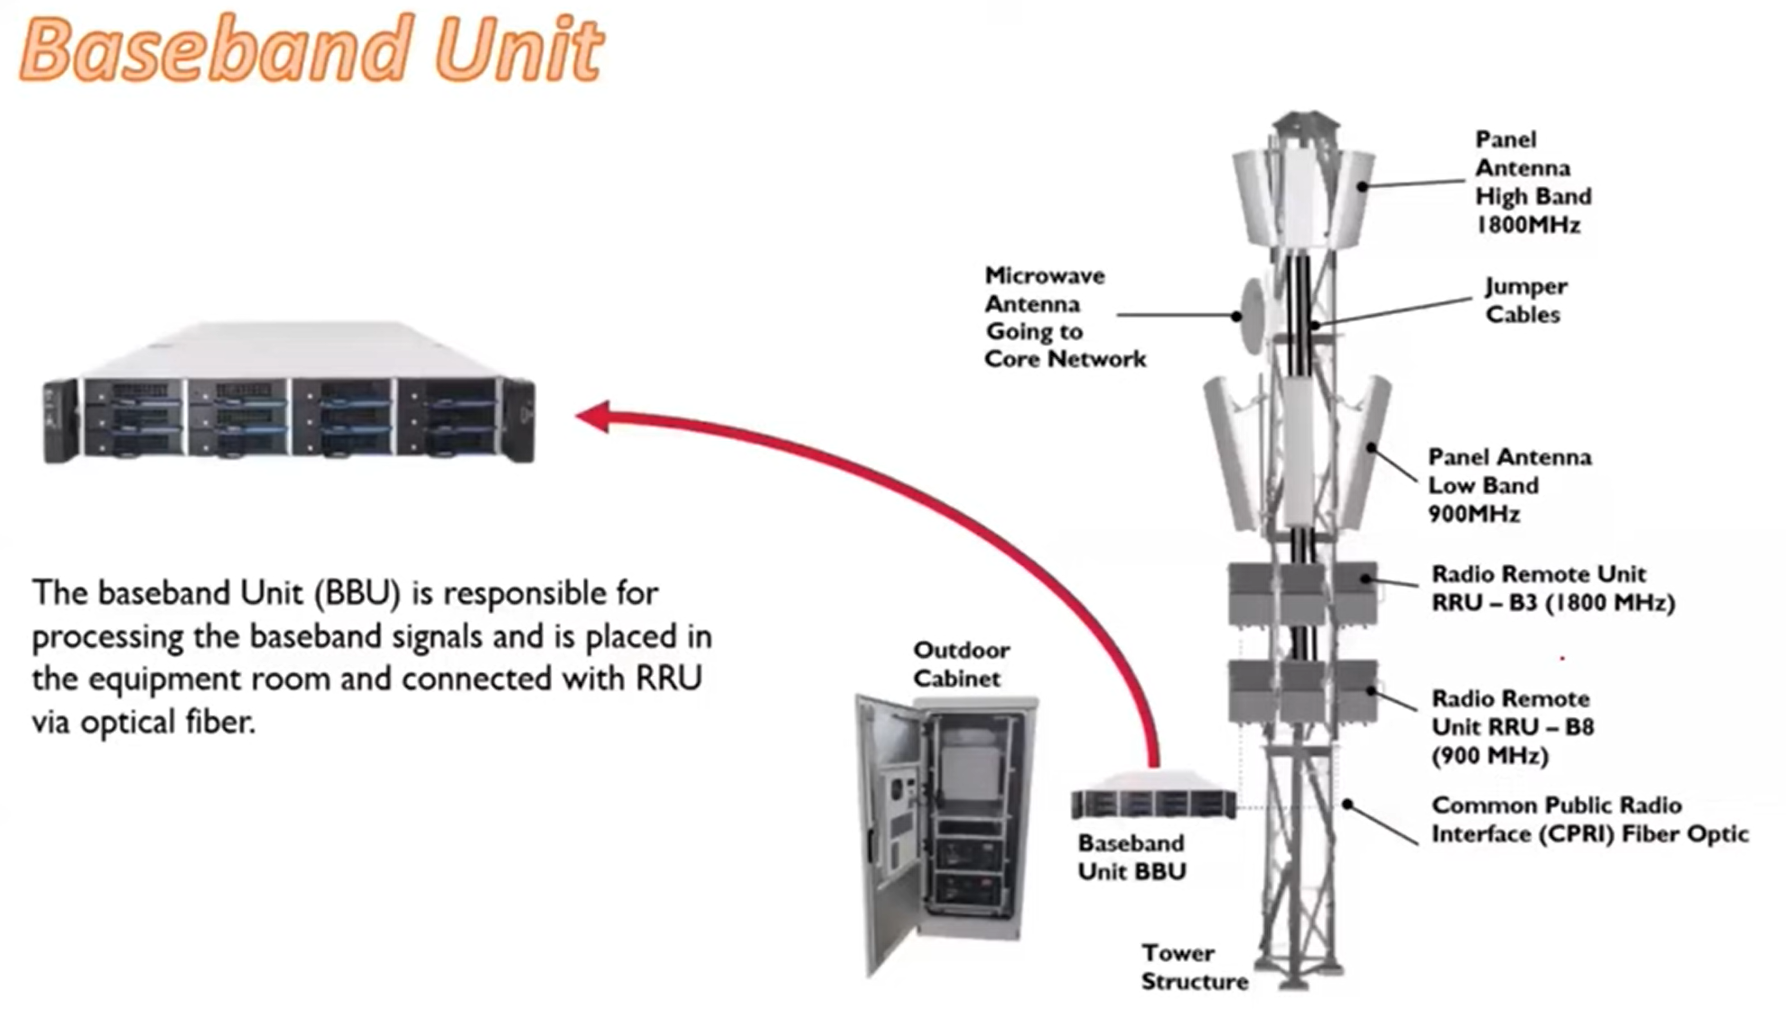
\includegraphics[width=.6\linewidth]{Pic/Baseband_Unit}
 	\caption{
 	\lr{Baseband}
 	در
 	\lr{Traditional RAN}
 	}
 	\label{fig:Baseband_Unit}
 \end{figure}

\section*{واحد
\lr{RRU}
}
واحد
 \lr{RU}
  یا
   \lr{RRU}
   (شکل \ref{fig:RRU}) روی برج نصب شده است . رابطی سریال به نام
     \lr{CPRI}
      ( 
    \lr{Common Public Radio Interface}
    ) که در شکل \ref{fig:CPRI} مشاهده می شود، انتقال داده ها با سرعت بالا از طریق کابل فیبر نوری را فراهم می‌سازد. درنتیجه از طریق آن تمامی سیگنال های رادیویی به
     \lr{function}
      محاسباتی (
       \lr{Computing Function}
       ) که در
        \lr{Base Band Unit}
         وجود دارد منتقل می‌شوند.
   
\begin{figure}[ht]
	\centering
	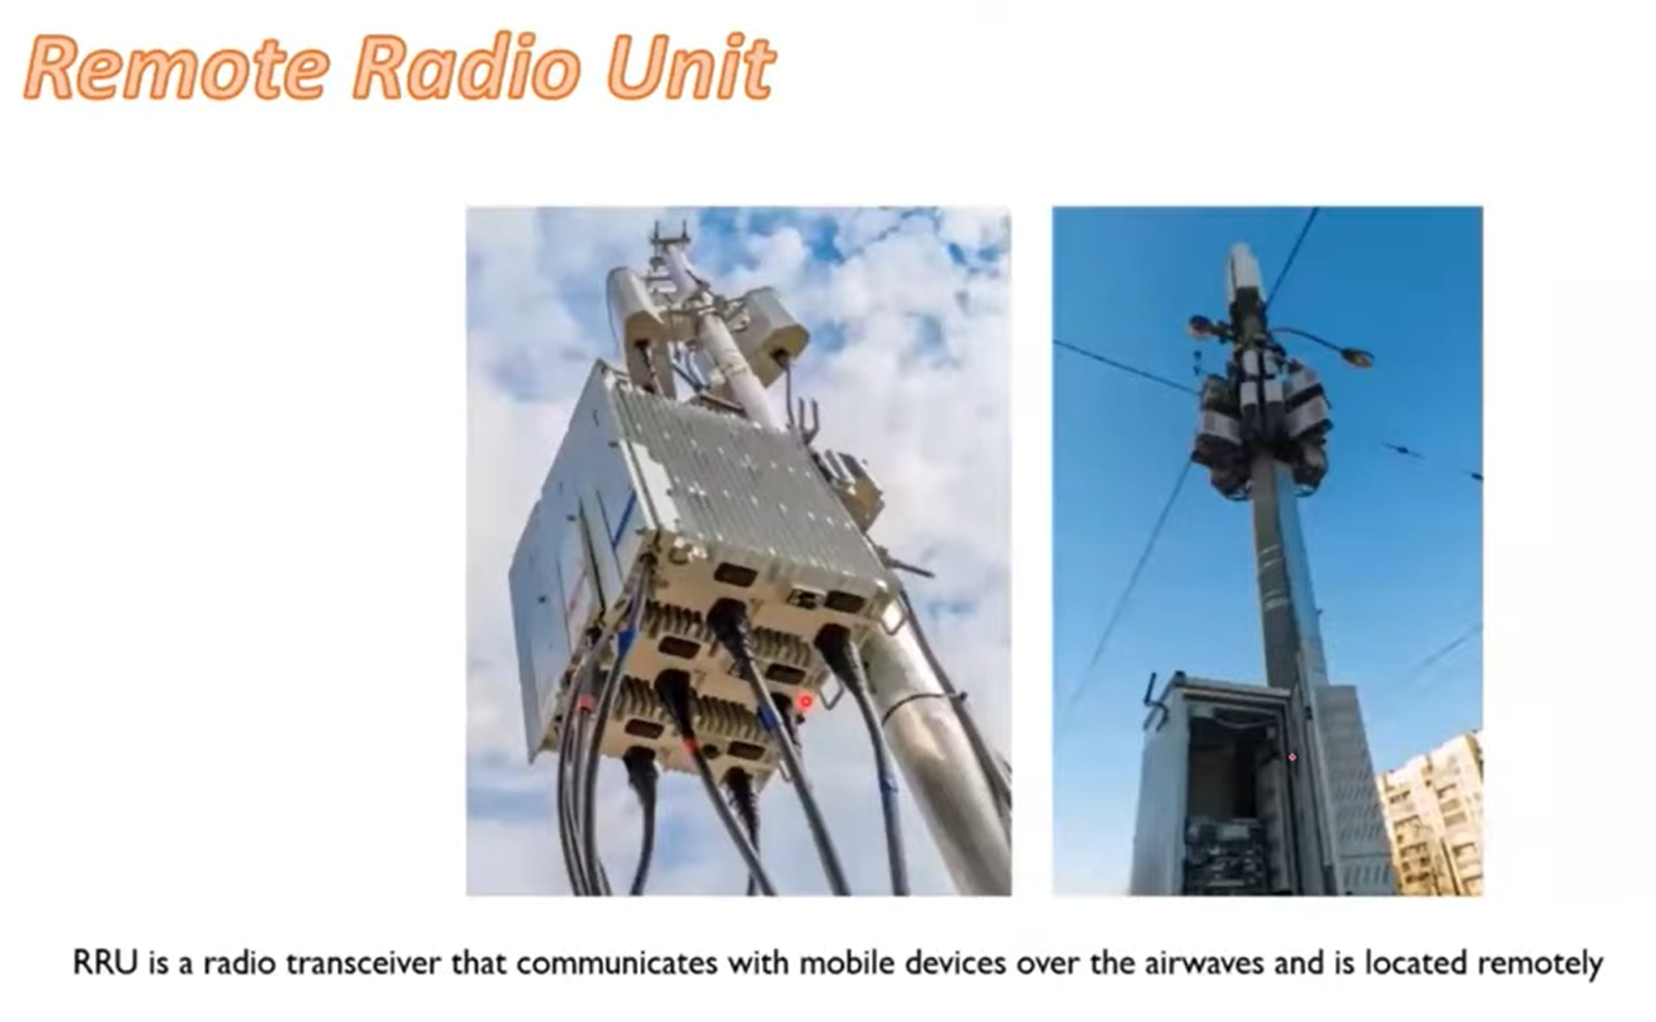
\includegraphics[width=.6\linewidth]{Pic/Remote_Radio_Unit}
	\caption{RRU}
	\label{fig:RRU}
\end{figure}

\begin{figure}[ht]
	\centering
	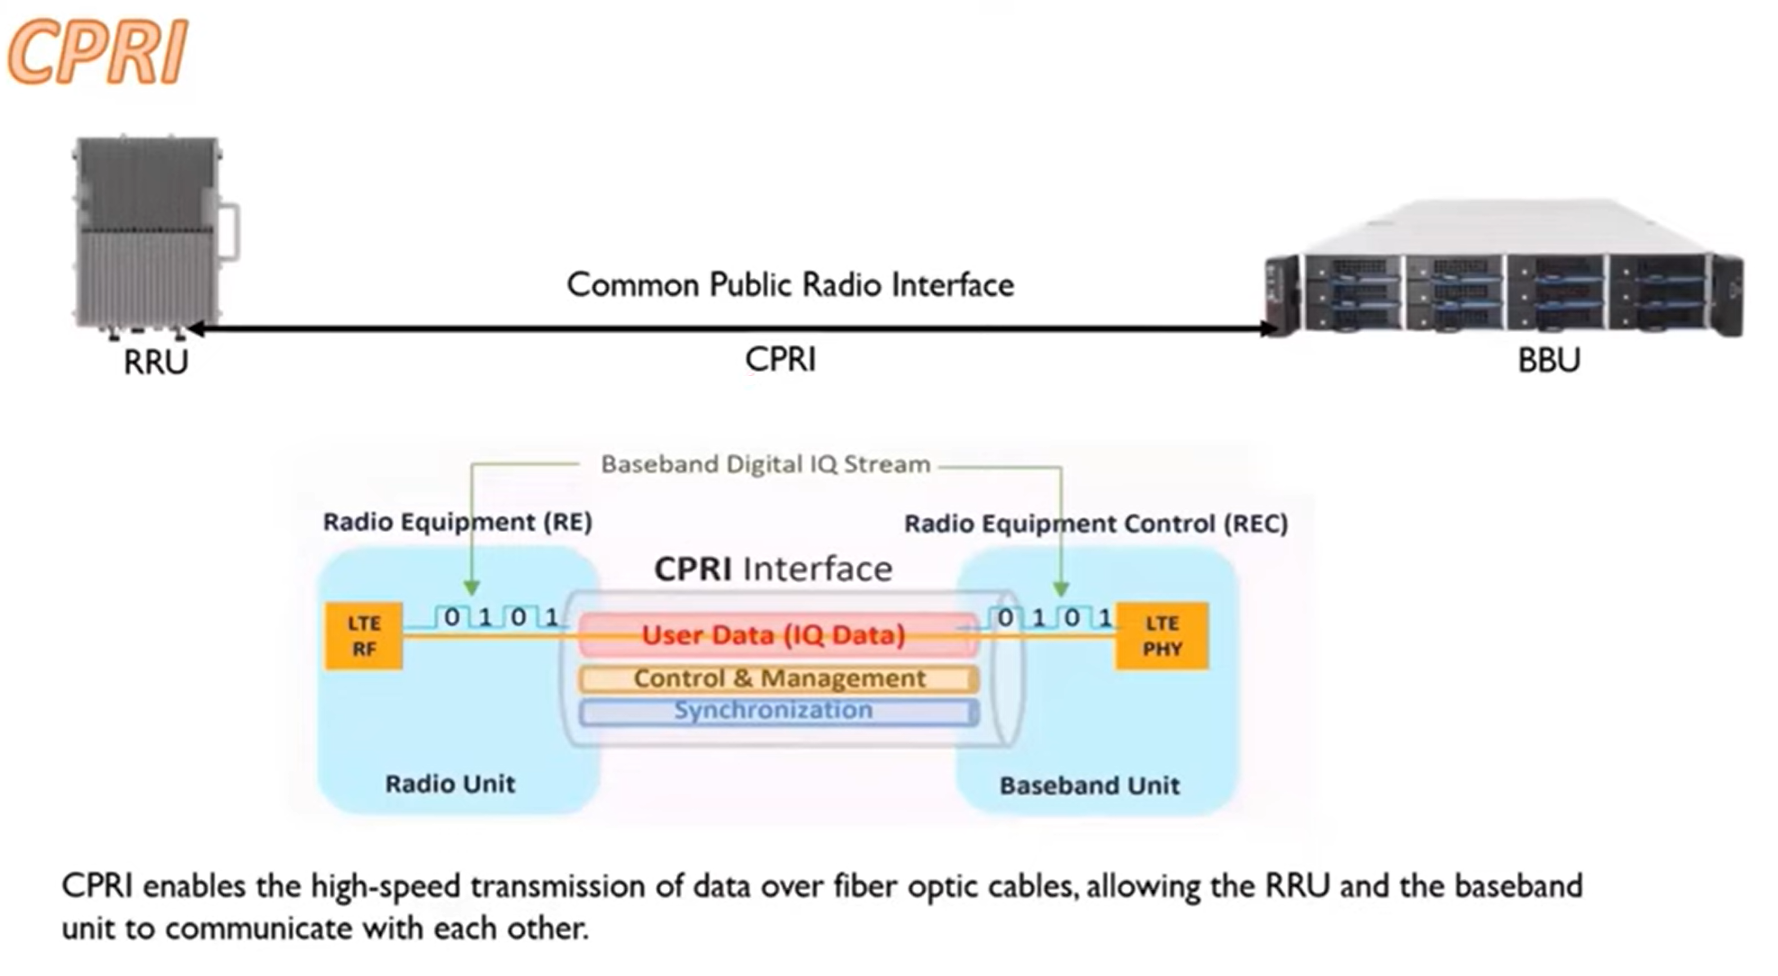
\includegraphics[width=.6\linewidth]{Pic/CPRI}
	\caption{CPRI}
	\label{fig:CPRI}
\end{figure}

در ناحیه
 \lr{RAN}
  به
   \lr{RRU}
    سخت افزار اختصاصی یا
     \lr{proprietary}
      می گویند و همچنین رابط میان
       \lr{RRU}
         و
          \lr{BBU}
           نیز اختصاصی و واحد
            \lr{BBU}
             خود شامل سخت افزار و نرم افزار اختصاصی است بدان معنا که اگر ما
              \lr{RRU}
               را از
                \lr{NOKIA}
                 خریداری کرده باشیم نمی‌توانیم
                  \lr{BBU}
                   را از
                    \lr{Ericsson}
                     خریداری کنیم.
                     
\chapter*{انواع
\lr{RAN}
}

\section*{CRAN}
به معنای
 \lr{Centralized RAN}
  است.
\section*{Virtual-RAN}                    
در حدود سال های 1994 ما دیوایس های مختلفی مثل رادیو،
 \lr{tape recorder}
 ، دوربین فیلم برداری،
  \lr{CD Player}
   و ... داشتیم و هم اکنون به کمک
    \lr{network function virtualization}
    گوشی همراه داریم و با کمک اپلیکیشن‌ها می‌توانیم عملکرد همان دستگاه ها را با کمک تلفن همراه داشته باشیم. به عبارتی ما به کمک
     \lr{NFV}
      ( 
    \lr{NETWORK FUNCTION VIRTUALIZATION} 
    ) از سخت افزار به نرم افزار گذر کردیم (شکل \ref{fig:vRAN})
    \begin{figure}[ht]
    	\centering
    	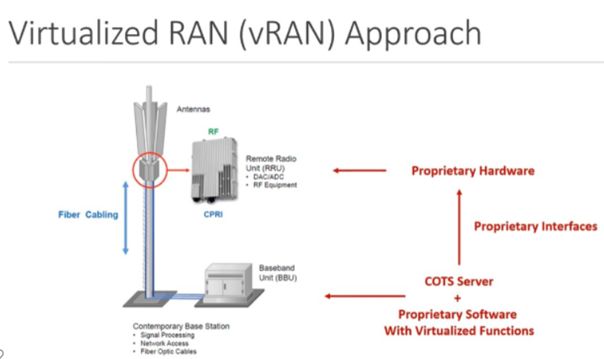
\includegraphics[width=.6\linewidth]{Pic/vRAN}
    	\caption{vRAN}
    	\label{fig:vRAN}
    \end{figure}
\section* {مراجع}
\begin{itemize}
	\item 
	\href{https://www.youtube.com/watch?v=Z9kJ8HT\_IVM} {ORAN}
	\item 
	\href{https://en.wikipedia.org/wiki/Radio_Interface_Layer} {RIL}
	
	\item 
	\href{https://en.wikipedia.org/wiki/Radio_Interface_Layer} {سوال اول}
	
	\item 
	\href{https://stackoverflow.com/questions/21170392/my-android-device-does-not-appear-in-the-list-of-adb-devices} {نمایش لیست دستگاه های 
	\lr{adb}
	}
	
	\item 
	\href{https://en-gb.support.motorola.com/app/answers/detail/a_id/159678/~/developer-options} {روشن کردن 
	\lr{Developer Mode}
	}
	
\end{itemize}

\end{document}
